\documentclass[xcolor=x11names, svgnames, rgb]{beamer}

\setbeamertemplate{navigation symbols}{}
\setbeamercolor{block title}{bg=blue!40}
\setbeamercolor{block body}{bg=blue!20}

%% Beamer Layout %%%%%%%%%%%%%%%%%%%%%%%%%%%%%%%%%%
\useoutertheme[subsection=false,shadow]{miniframes}
\useinnertheme{default}
\usefonttheme{serif}
\usepackage{palatino}
\setbeamerfont{title like}{shape=\scshape}
\setbeamerfont{frametitle}{shape=\scshape}
\setbeamercolor*{lower separation line head}{bg=DeepSkyBlue4}
\setbeamercolor*{normal text}{fg=black,bg=white}
\setbeamercolor*{alerted text}{fg=red}
\setbeamercolor*{example text}{fg=black}
\setbeamercolor*{structure}{fg=black}
\setbeamercolor*{palette tertiary}{fg=black,bg=black!10}
\setbeamercolor*{palette quaternary}{fg=black,bg=black!10}
%% END Beamer Layout %%%%%%%%%%%%%%%%%%%%%%%%%%%%%%%%%%%%%%%%%%%%
\usepackage{graphicx}
\usepackage{algpseudocode}
\usepackage{soul}

\usepackage{mathtools}
\newcommand{\defeq}{\vcentcolon=}
\DeclarePairedDelimiter{\paren}{(}{)}

\newcommand{\dec}{\operatorname{dec}}
\newcommand{\poly}{\operatorname{poly}}
\newcommand{\polylog}{\operatorname{polylog}}
\newcommand{\github}{\url{github.com/awestover/Parallel-Partition}}
\newcommand{\defn}[1]       {{\textit{\textbf{\boldmath #1}}}}
\newcommand{\paragraph}[1]{\vspace{0.09in}\noindent{\bf \boldmath #1.}} 
\usepackage{amsmath}
\def\E{\operatorname{\mathbb{E}}}
\usepackage{amssymb}
\usepackage{amsthm}

\newtheorem{proposition}{Proposition}
\newtheorem{defin}{Definition}
\newtheorem{conj}{Conjecture}

\usepackage{hyperref}

\usepackage{tikz,pgfplots}
\usepackage{etoolbox}
%% This makes the colors annoyingly bright, but at least they're easy to distinguish.
\pgfplotsset{
  every  tick/.style={red,}, minor x tick num=1,
  cycle list={teal,every mark/.append style={fill=teal!80!black},mark=*\\%
orange,every mark/.append style={fill=orange!80!black},mark=square*\\%
cyan!60!black,every mark/.append style={fill=cyan!80!black},mark=otimes*\\%
red!70!white,mark=star\\%
lime!80!black,every mark/.append style={fill=lime},mark=diamond*\\%
red,densely dashed,every mark/.append style={solid,fill=red!80!black},mark=*\\%
yellow!60!black,densely dashed,
every mark/.append style={solid,fill=yellow!80!black},mark=square*\\%
black,every mark/.append style={solid,fill=gray},mark=otimes*\\%
blue,densely dashed,mark=star,every mark/.append style=solid\\%
red,densely dashed,every mark/.append style={solid,fill=red!80!black},mark=diamond*\\%
}
}
\pgfplotsset{compat=1.6}


\usepackage{xcolor}
\newcommand{\citefont}[1]{{\tiny \textcolor{Gray}{#1}}}


\title{Variable Processor Cup Games}
\author{Alek Westover}
\institute{Belmont High School}
\date{June 1, 2020}

\begin{document}
 
\frame{\titlepage}

\begin{frame}[t]{What is the Cup Game?}
  \begin{definition}
  The \defn{$p$-processor cup-game} on $n$ cups is a multi-round game in which
  two players take turns emptying and removing water from the cups. \\
  On each round
  \begin{itemize}
    \item The \defn{filler} distributes $p$ units of water among the cups (with at most $1$ unit to any particular cup). 
    \item Then the \defn{emptier} chooses $p$ cups to remove (at most) one unit of water from.
  \end{itemize}
  \end{definition}
\end{frame}

\begin{frame}[t]{What is the Cup Game?}
  \begin{definition}
  The \defn{backlog} of the system is the amount of water in the fullest cup;
  The emptier aims to minimize backlog whereas the filler aims to maximize
  backlog.
  \end{definition}
  \vspace{0.4cm}

  \textbf{Note:} The emptier's resources must be allocated discretlely whereas
  the filler can continuously distribute resources.
\end{frame}


\begin{frame}[t]{Why is it important?}
  The cup game models \defn{work scheduling}:
  \begin{itemize}
    \item The $n$ cups represent tasks that must be performed. 
    \item At each time step:
      \begin{itemize}
        \item $p$ new units of work come in, distributed
          arbitrarily among the $n$ tasks (with the constraint that no task gets
          more than $1$ unit of work) 
        \item $p$ processors must be allocated to a subset the
          tasks, on which they will achieve $1$ unit of progress.
      \end{itemize}
\end{itemize}

  \vspace{0.5cm}
  The cup game is also an interesting mathematical object.
\end{frame}

\begin{frame}[t]{Single-Processor Lower Bound}
  \textbf{Filling strategy}: distribute water equally amongst cups not yet emptied by the emptier.
  \vspace{0.3cm}

  \begin{overprint}
    \onslide<1>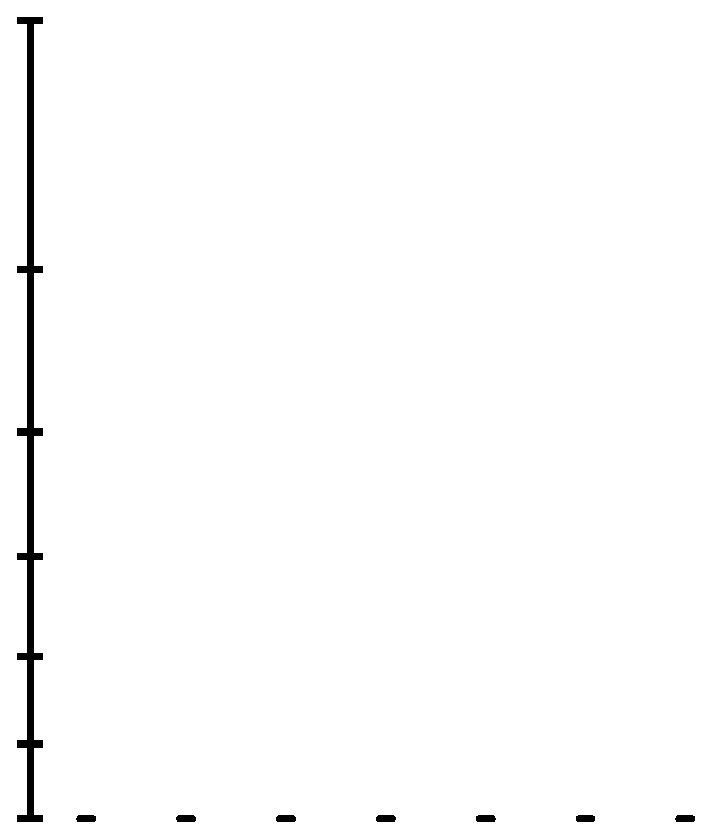
\includegraphics[width=0.5\linewidth]{singleProcessorLowerBound/round_0_1.eps}
    \onslide<2>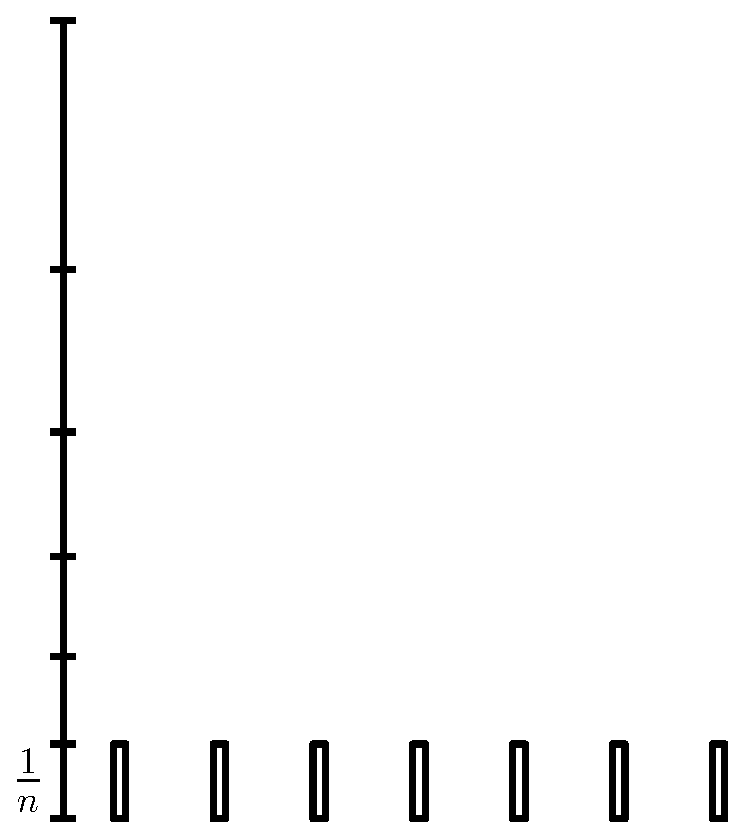
\includegraphics[width=0.5\linewidth]{singleProcessorLowerBound/round_1_0.eps}
    \onslide<3>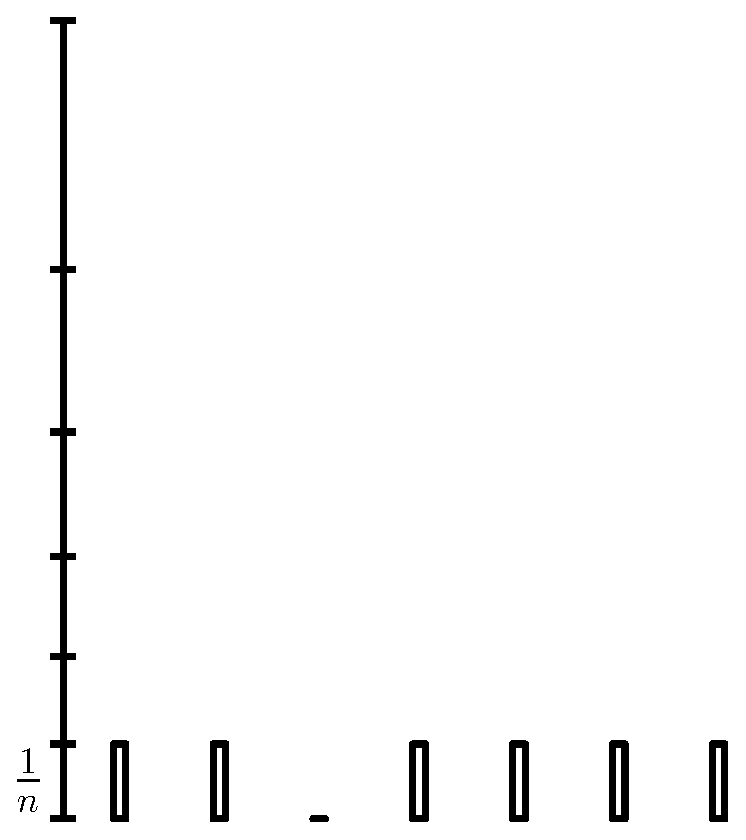
\includegraphics[width=0.5\linewidth]{singleProcessorLowerBound/round_1_1.eps}
    \onslide<4>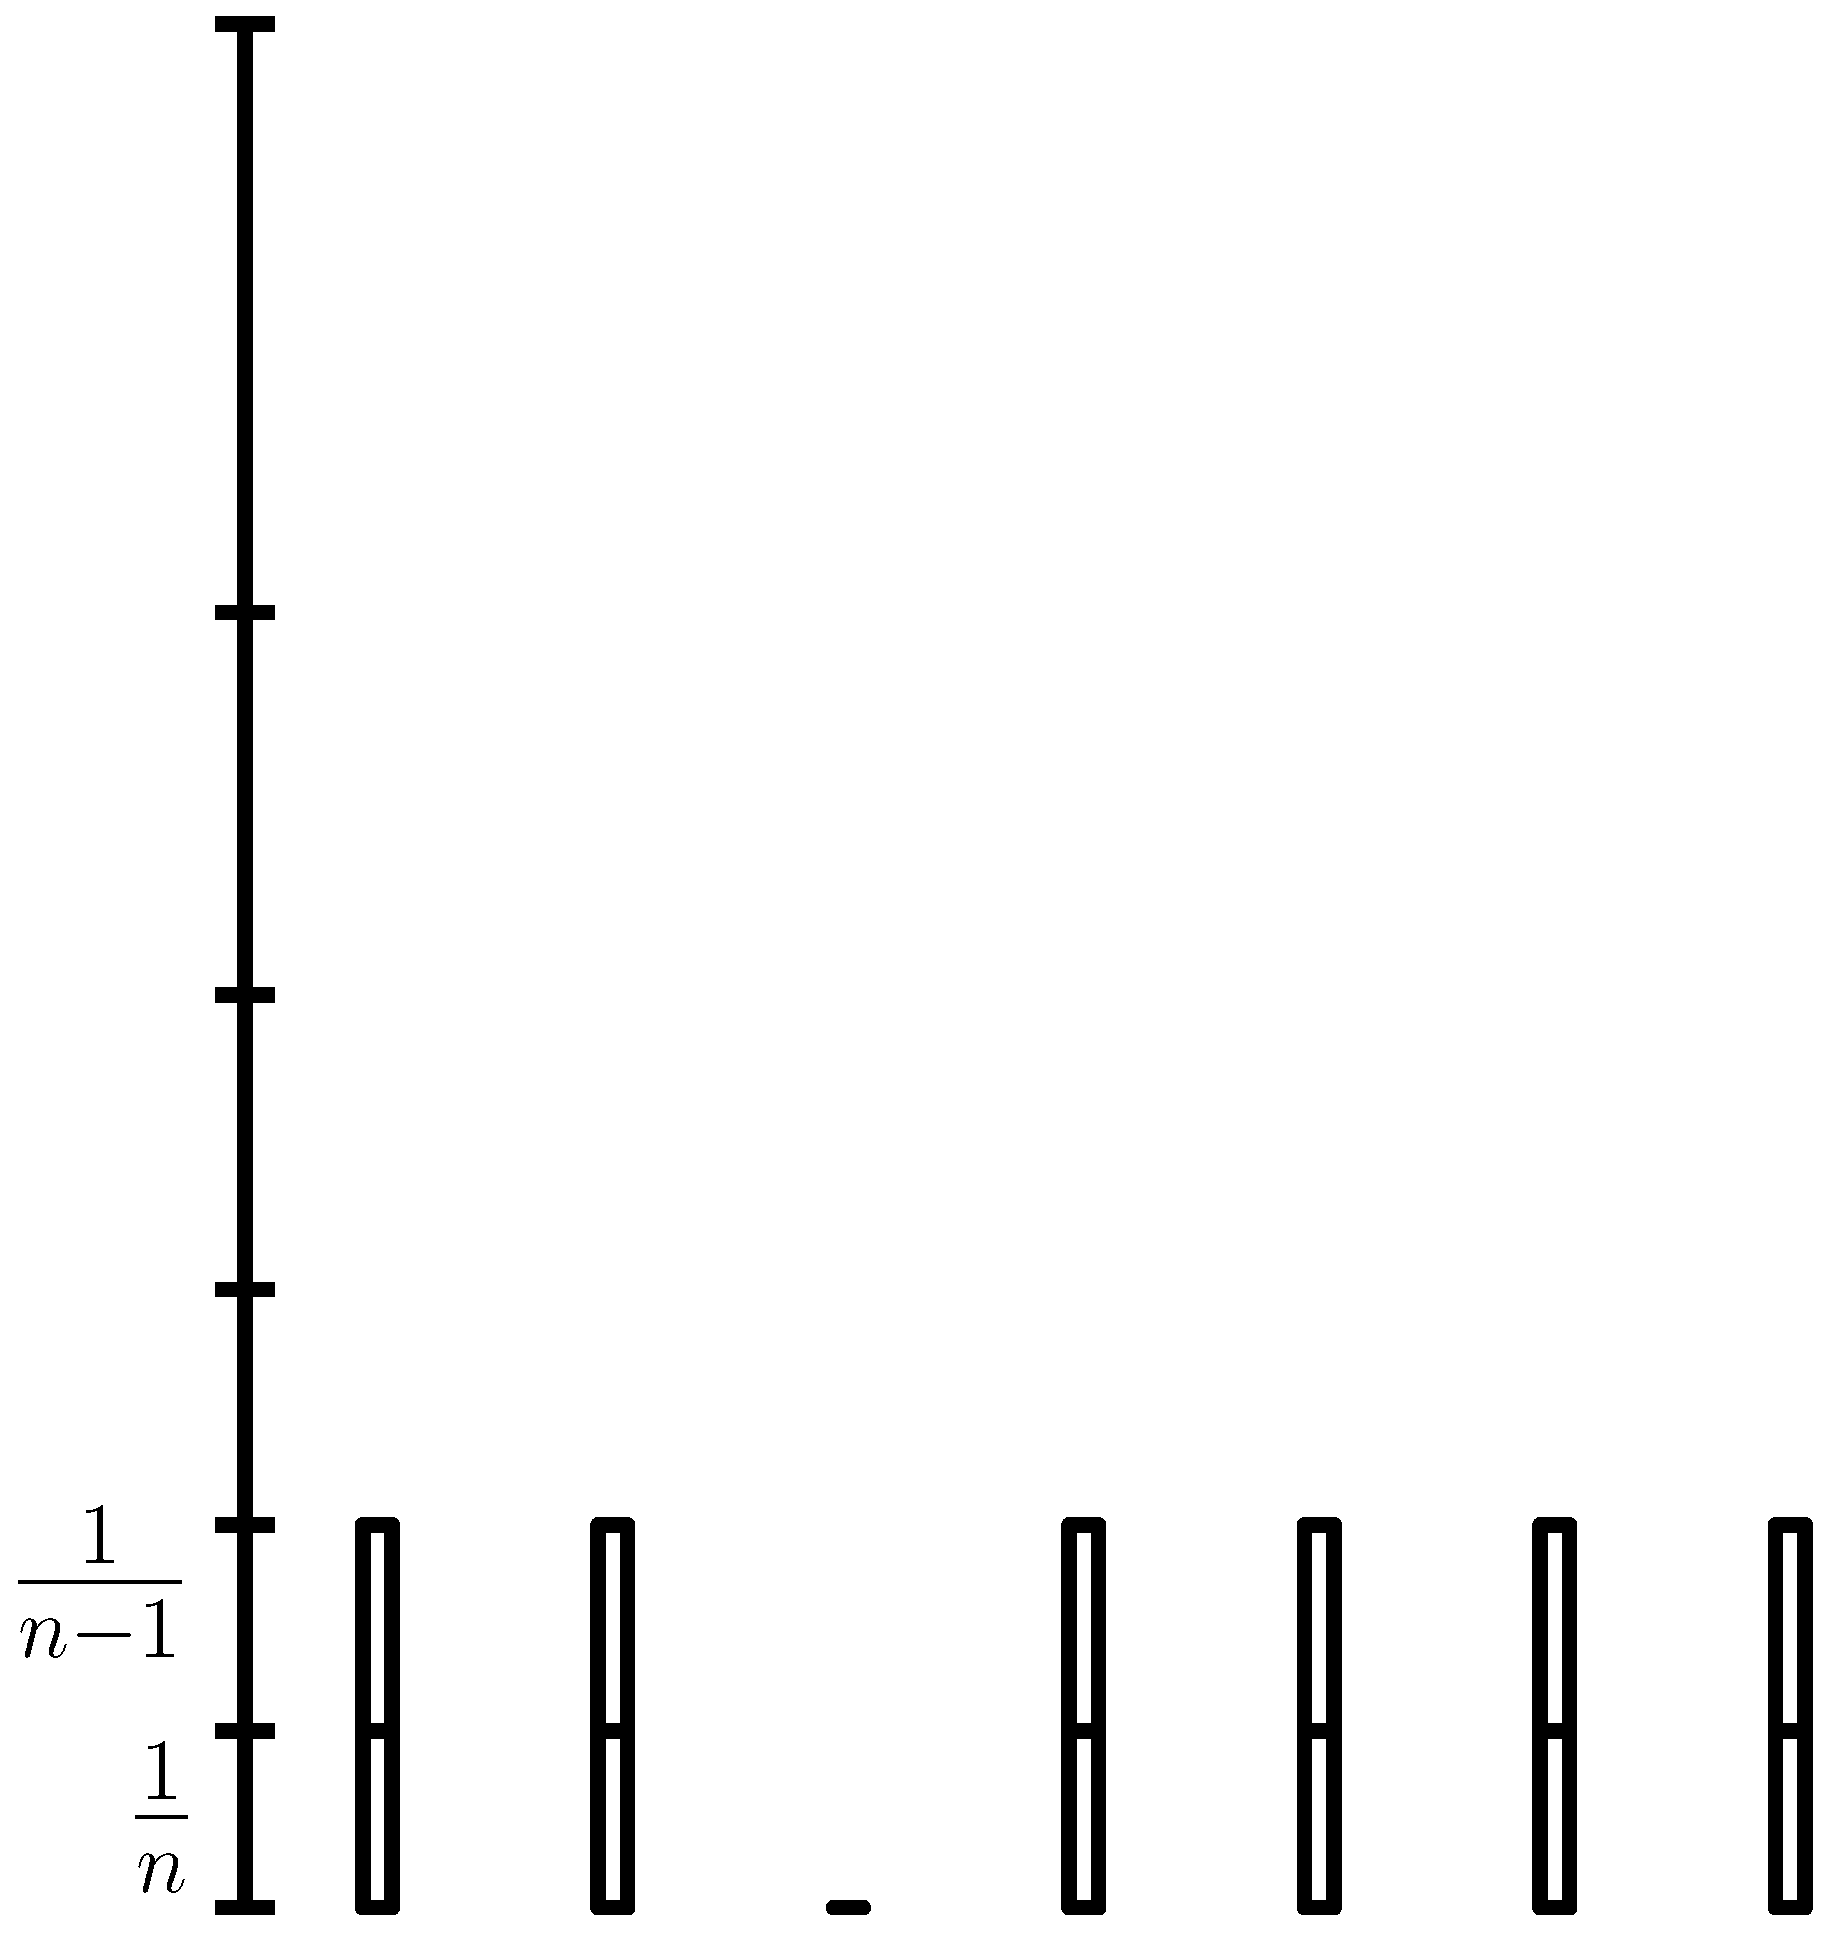
\includegraphics[width=0.5\linewidth]{singleProcessorLowerBound/round_2_0.eps}
    \onslide<5>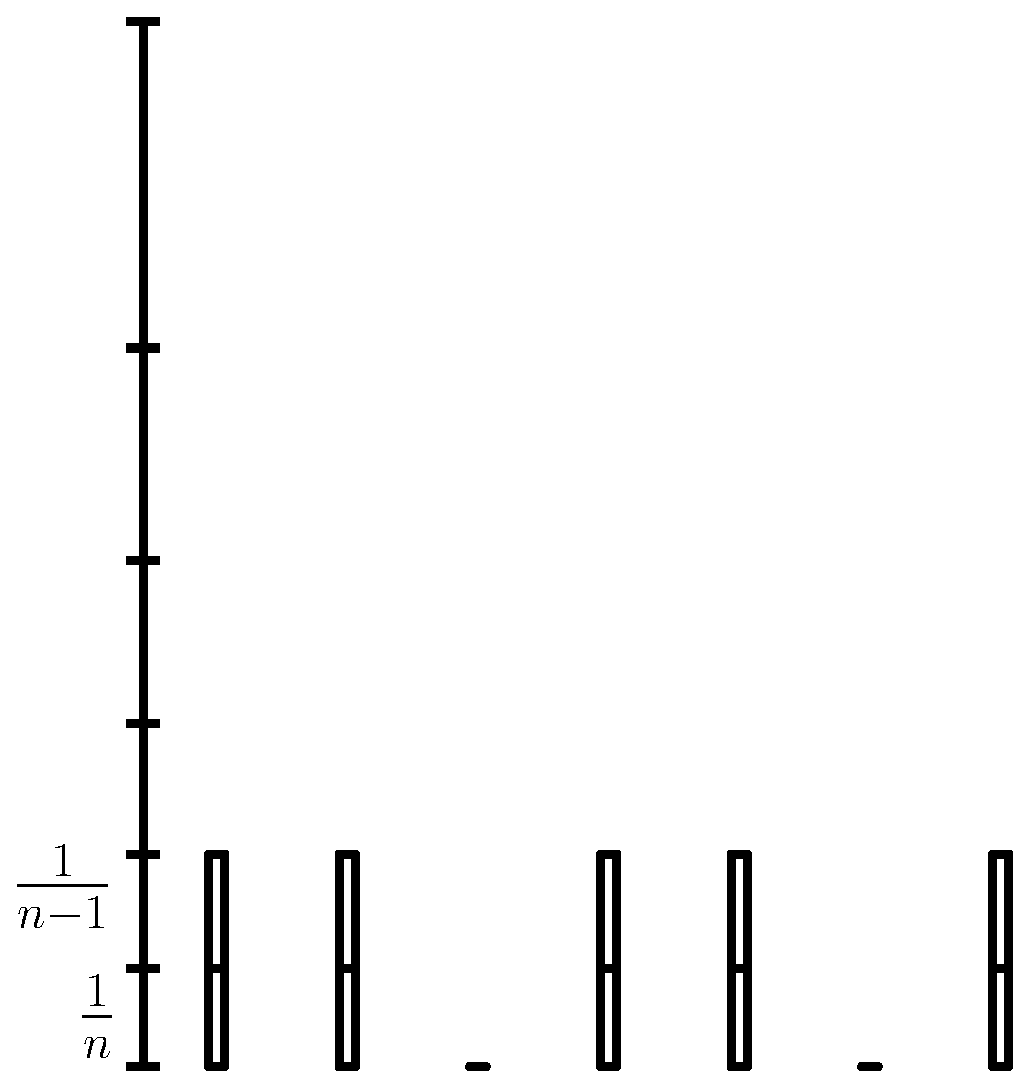
\includegraphics[width=0.5\linewidth]{singleProcessorLowerBound/round_2_1.eps}
    \onslide<6>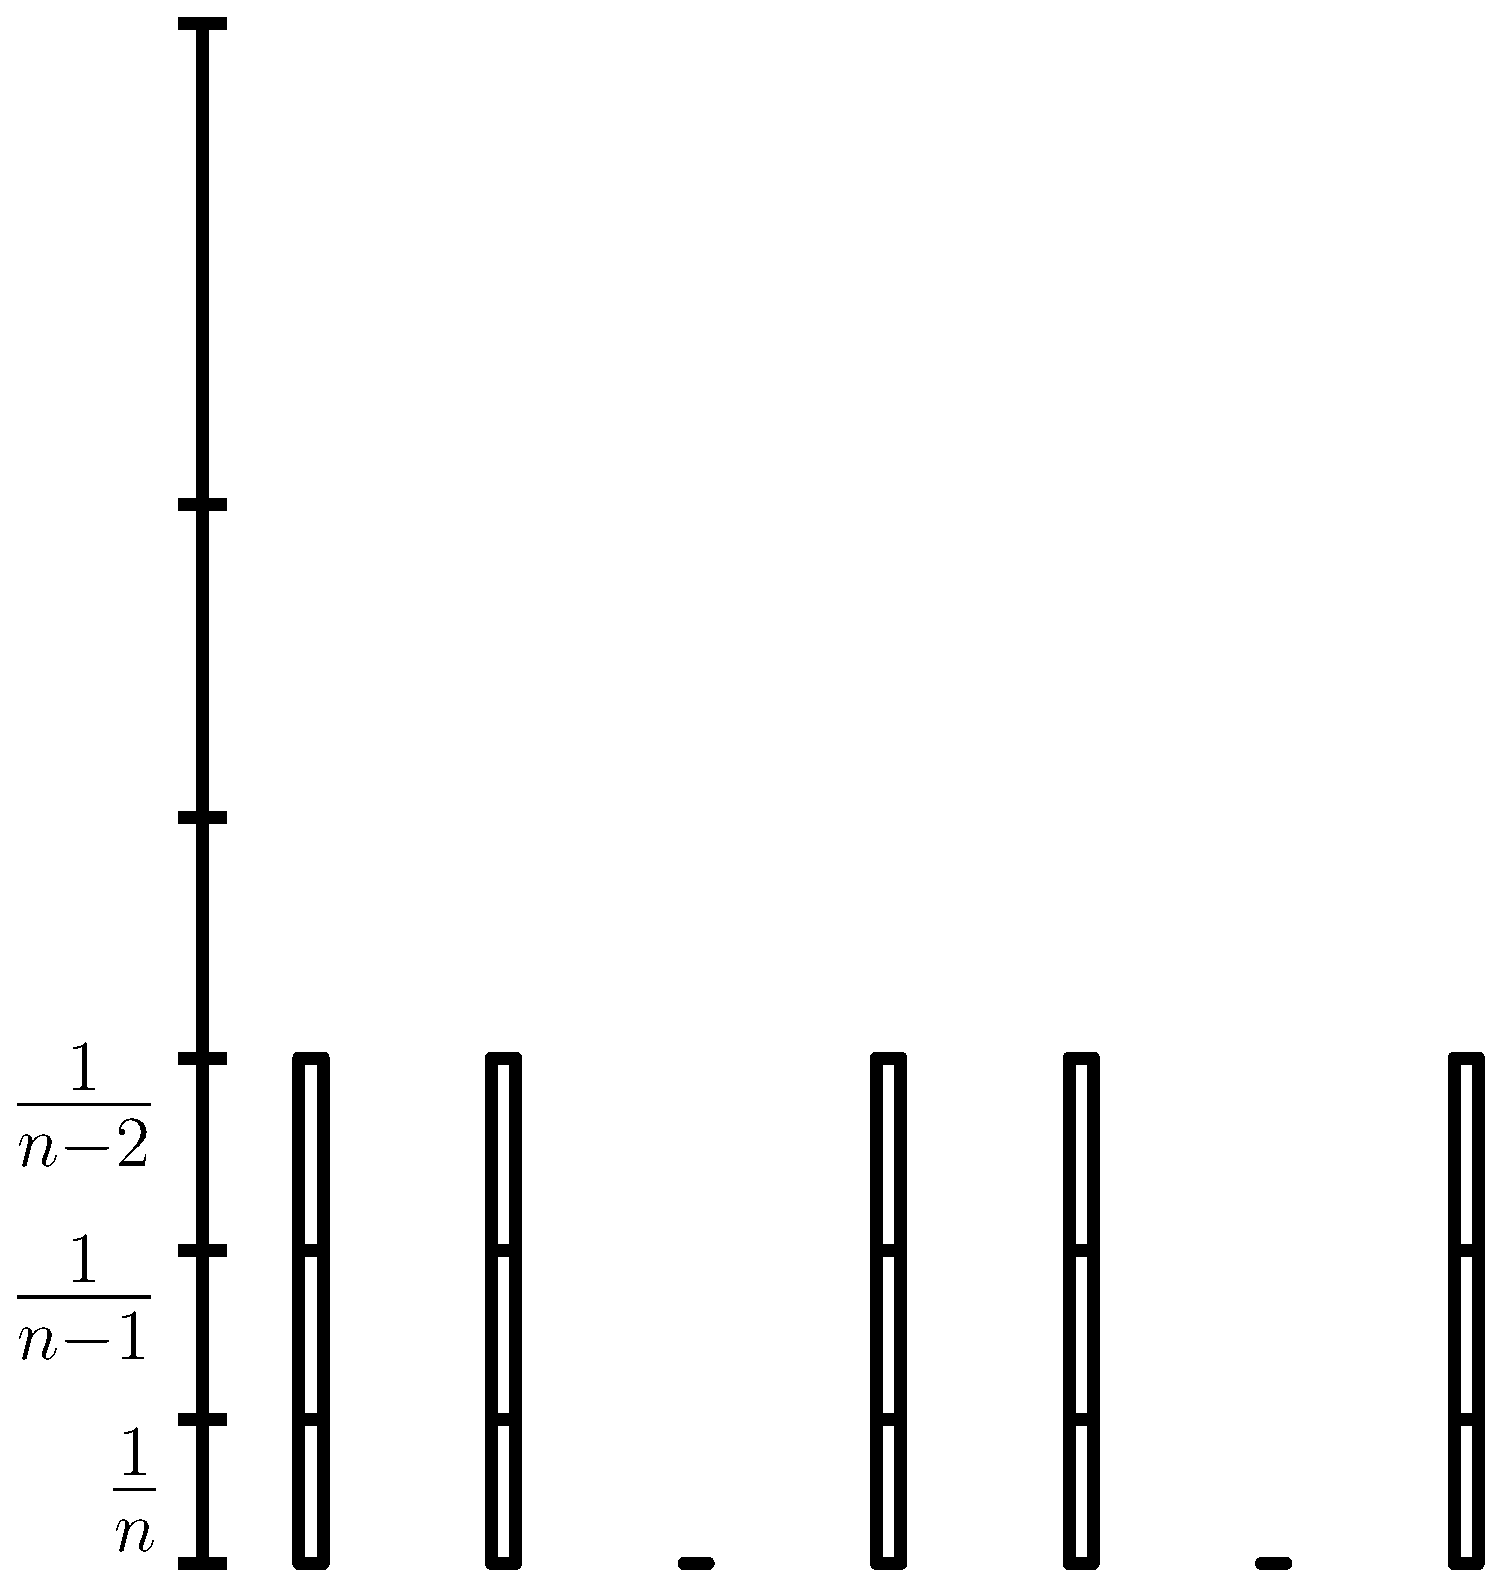
\includegraphics[width=0.5\linewidth]{singleProcessorLowerBound/round_3_0.eps}
    \onslide<7>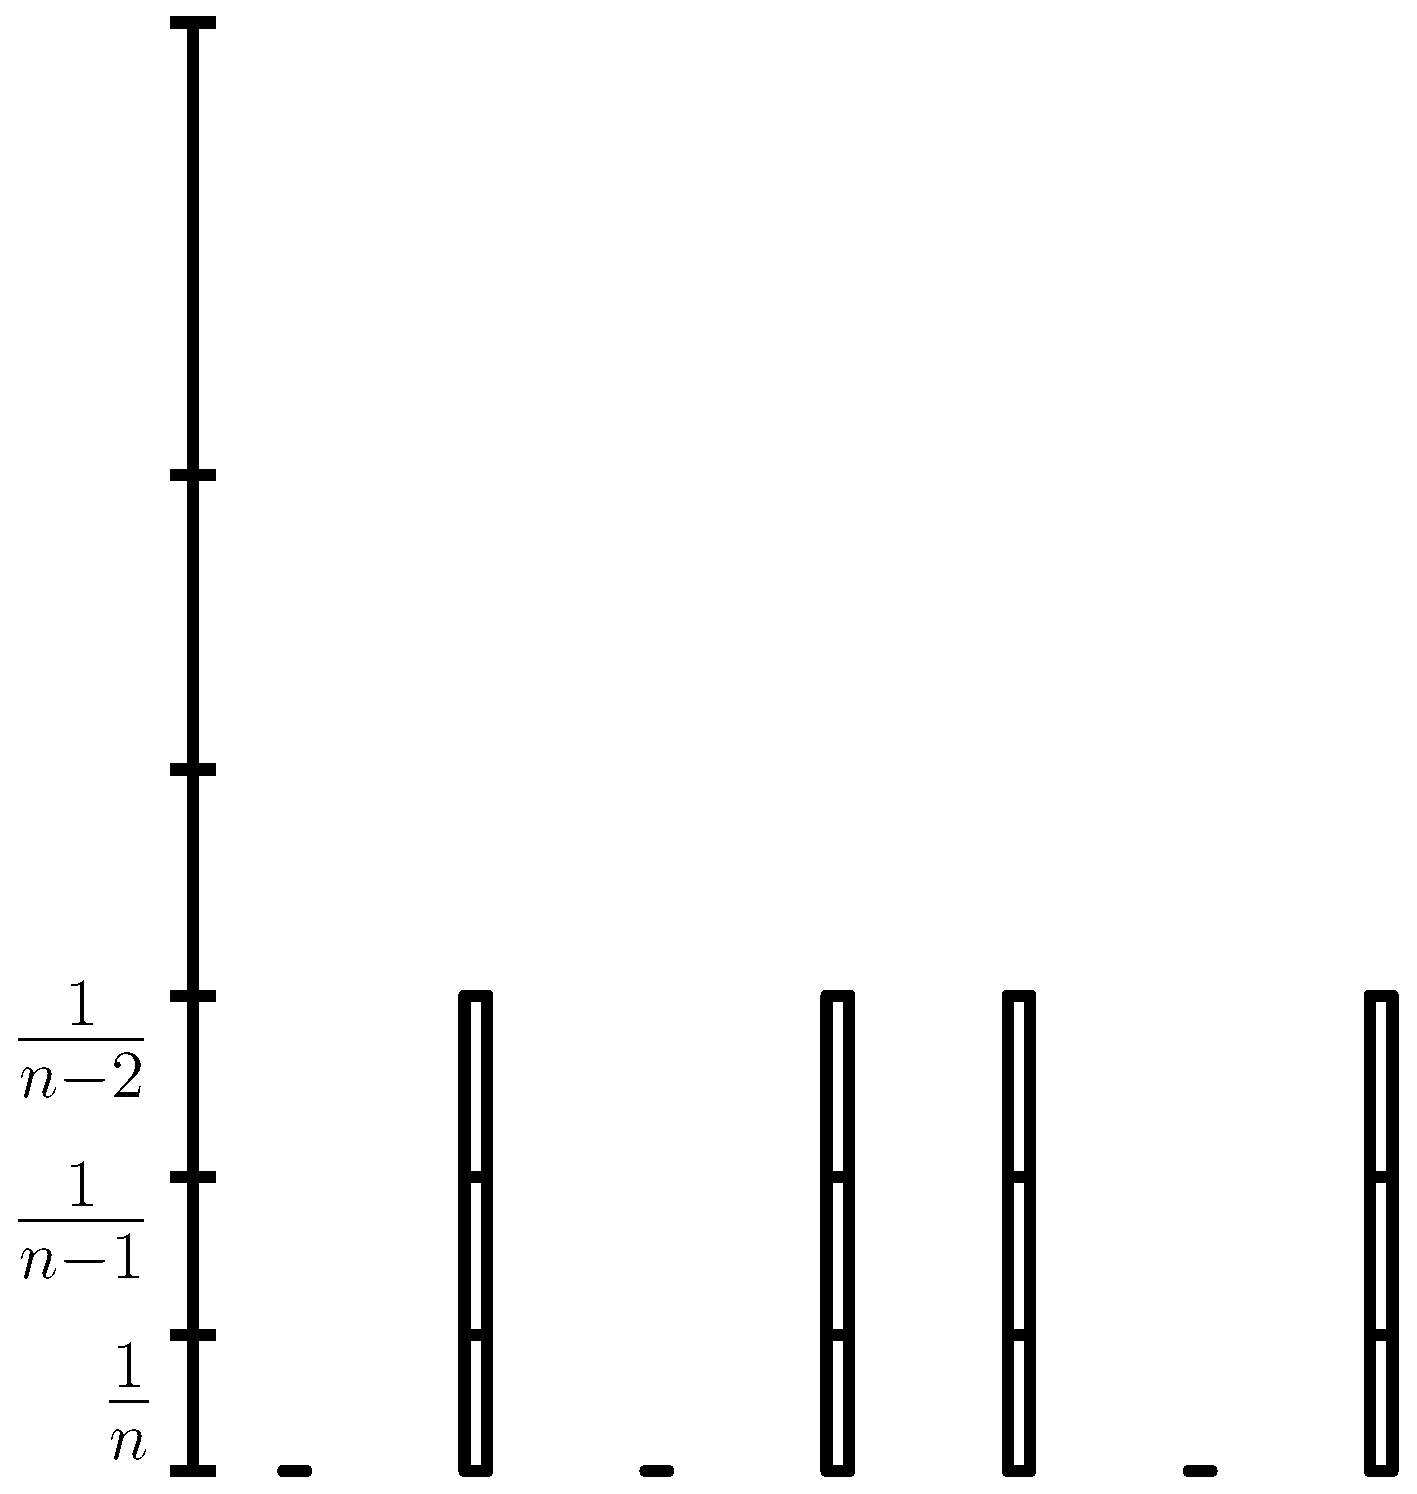
\includegraphics[width=0.5\linewidth]{singleProcessorLowerBound/round_3_1.eps}
    \onslide<8>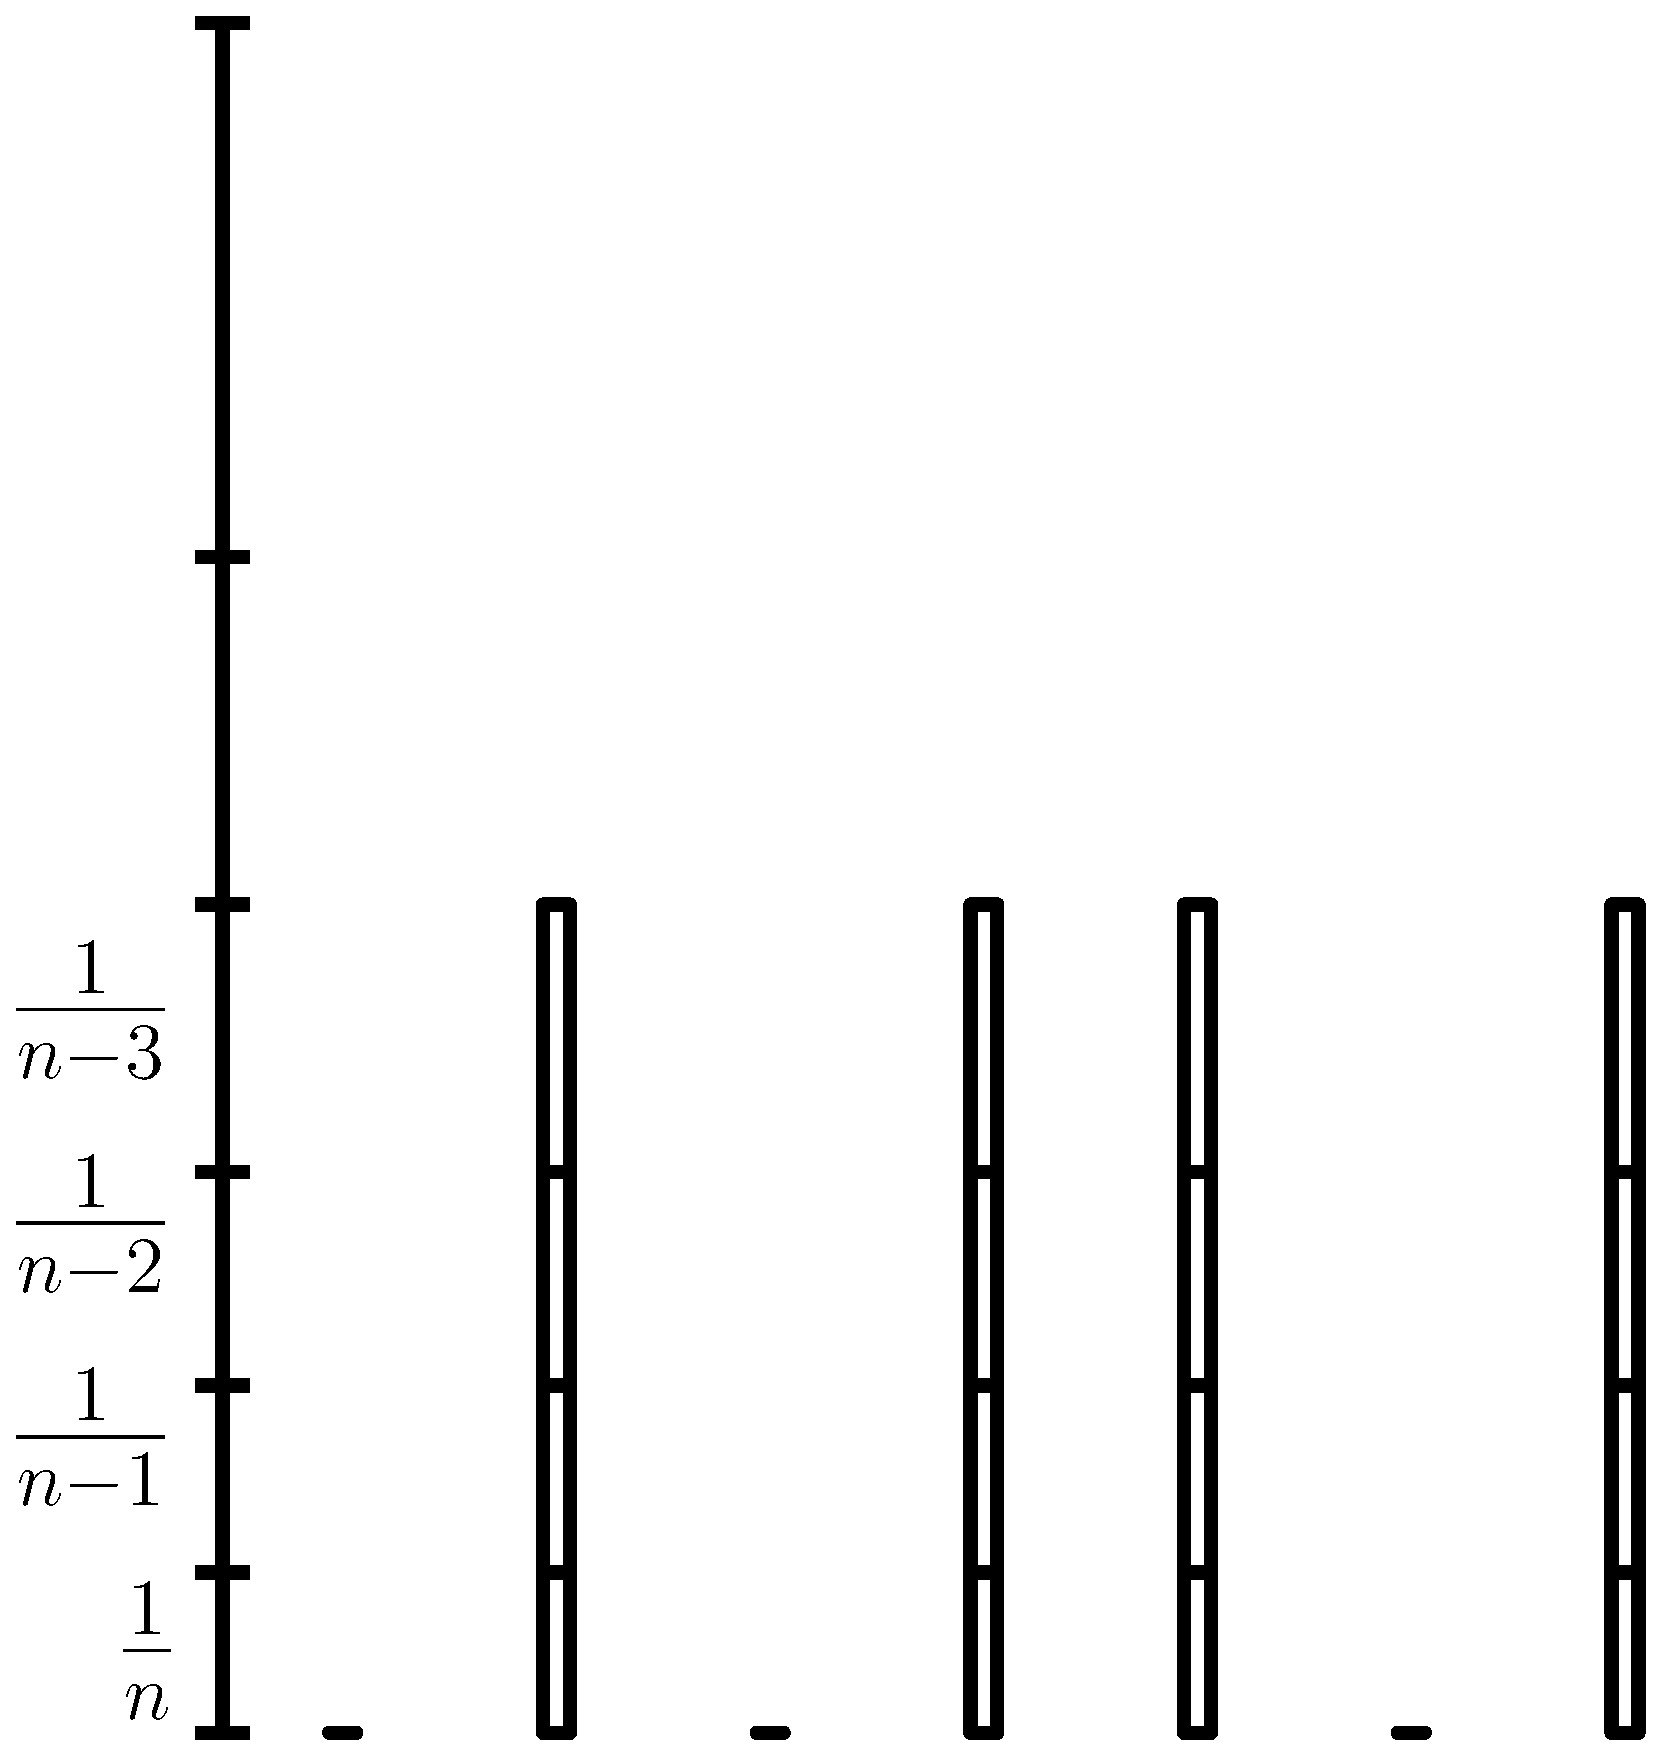
\includegraphics[width=0.5\linewidth]{singleProcessorLowerBound/round_4_0.eps}
    \onslide<9>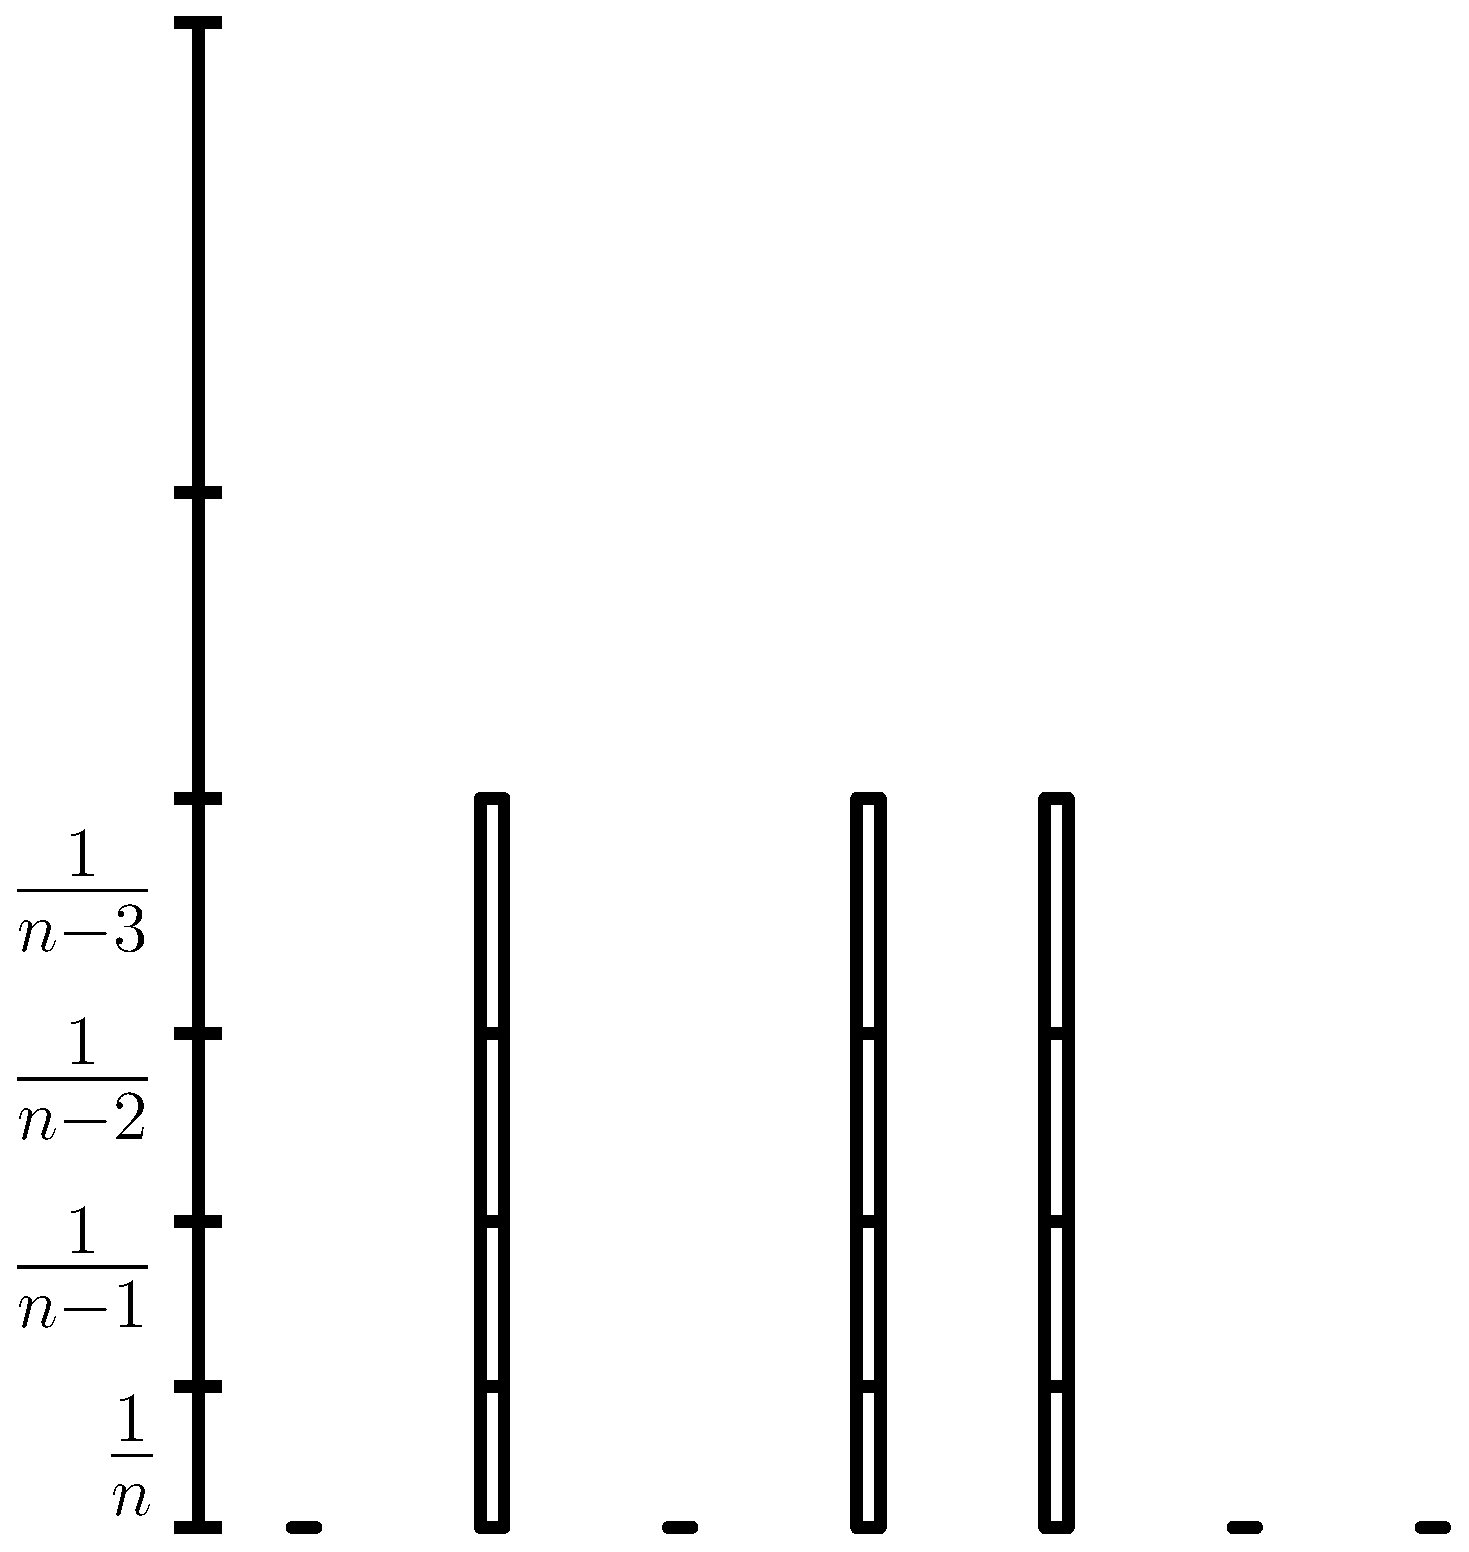
\includegraphics[width=0.5\linewidth]{singleProcessorLowerBound/round_4_1.eps}
    \onslide<10>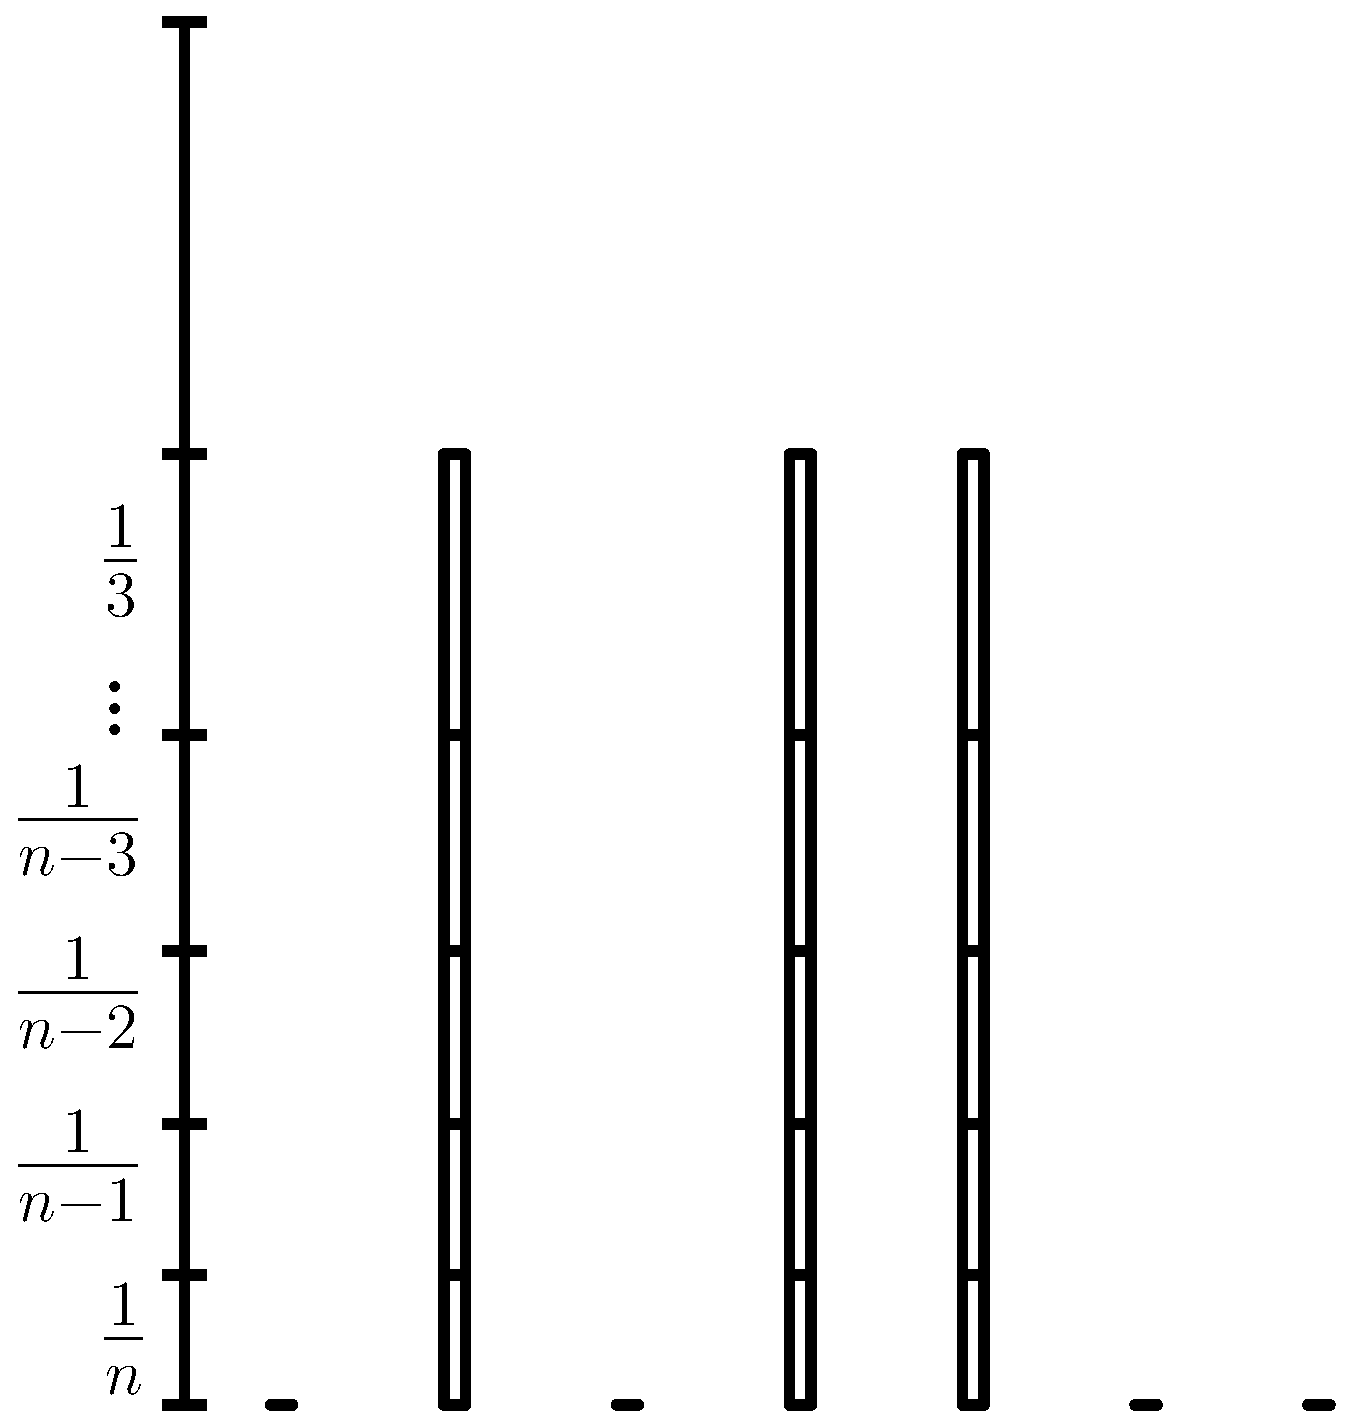
\includegraphics[width=0.5\linewidth]{singleProcessorLowerBound/round_5_0.eps}
    \onslide<11>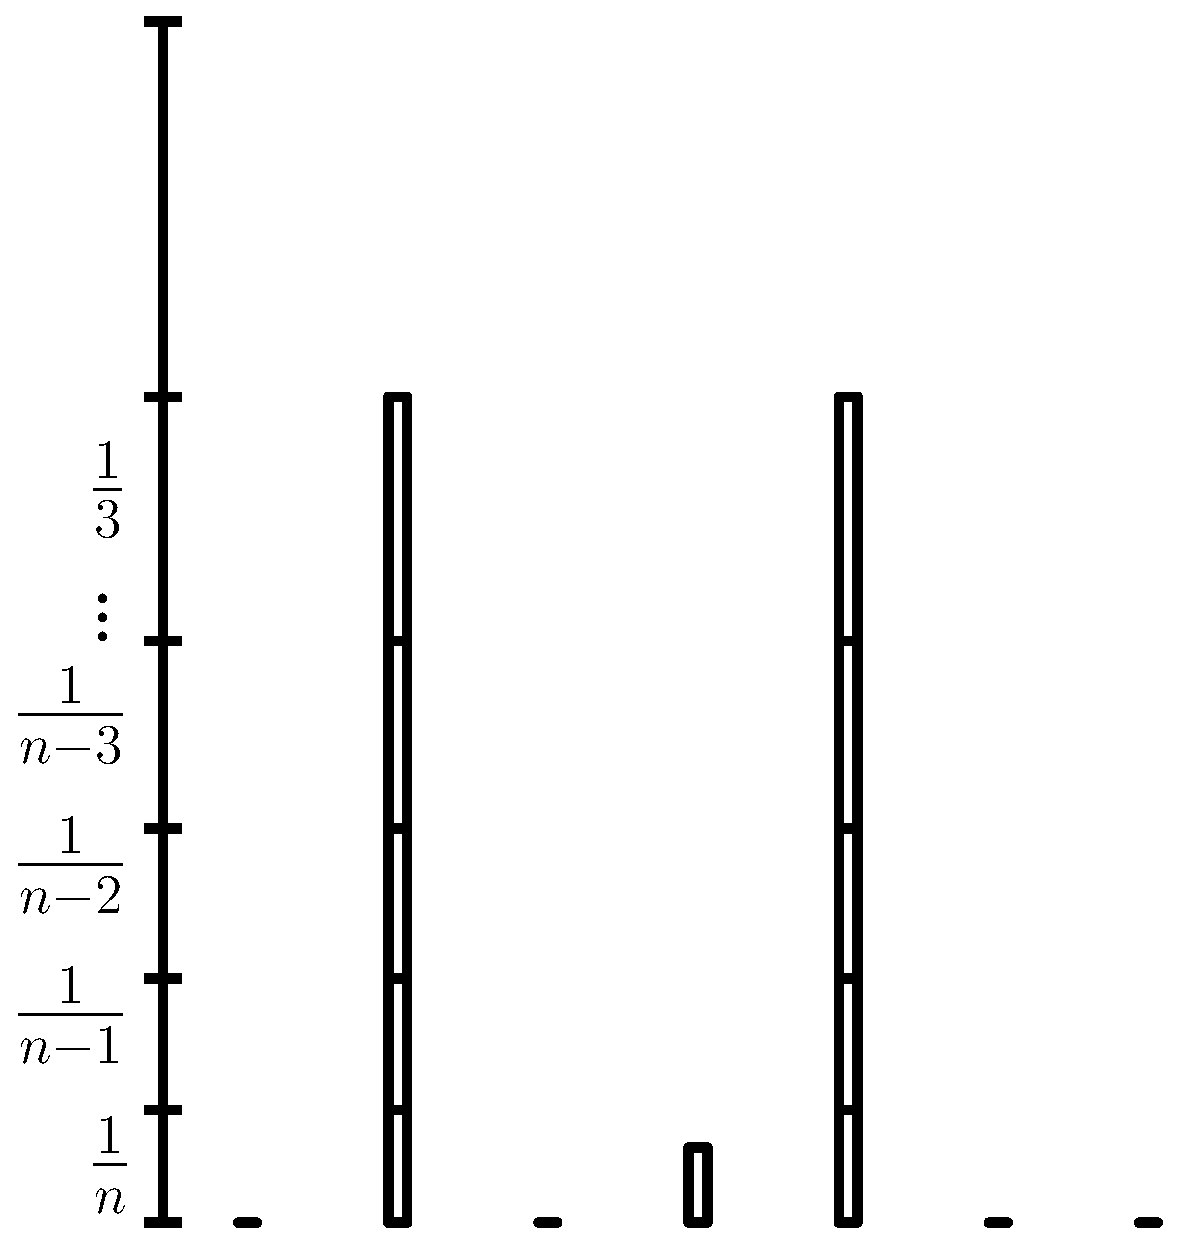
\includegraphics[width=0.5\linewidth]{singleProcessorLowerBound/round_5_1.eps}
    \onslide<12>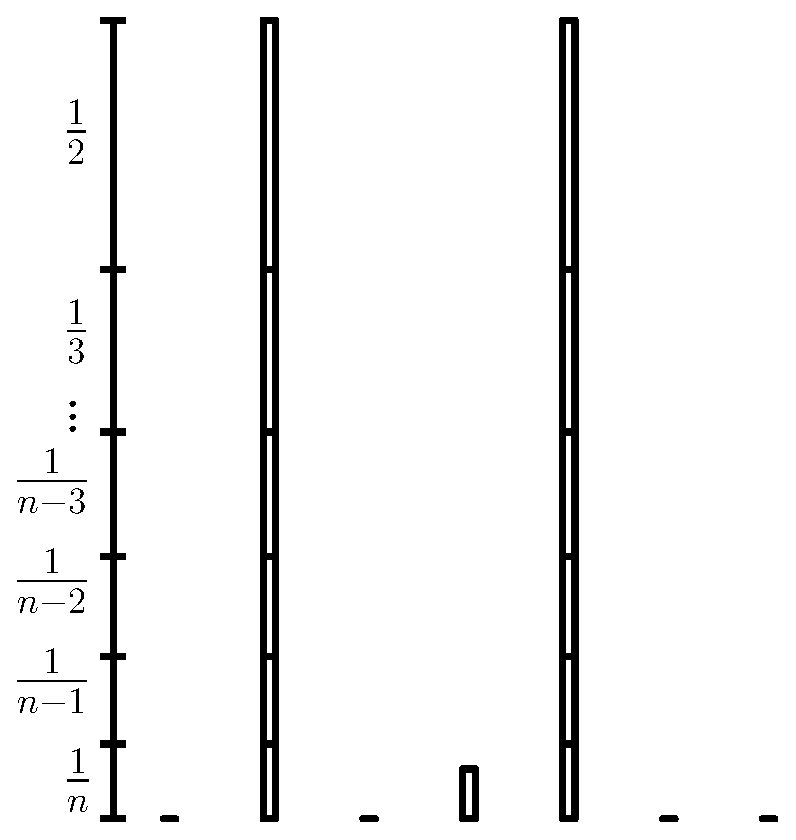
\includegraphics[width=0.5\linewidth]{singleProcessorLowerBound/round_6_0.eps}
    \onslide<13>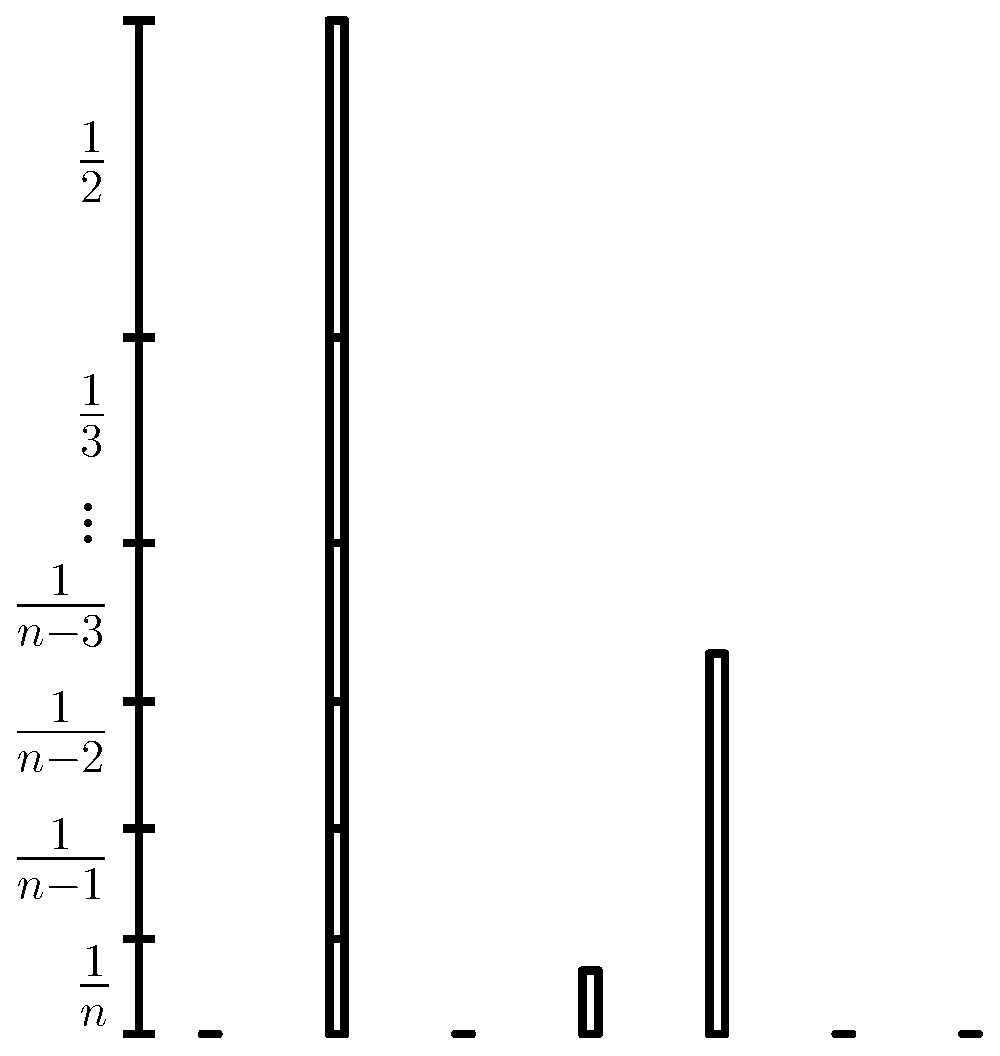
\includegraphics[width=0.5\linewidth]{singleProcessorLowerBound/round_6_1.eps}
    \onslide<14>\vspace{1.5cm}Achieves backlog: $$\frac{1}{n} + \frac{1}{n-1} + \cdots + \frac{1}{2} = \Omega(\log n).$$ 
  \end{overprint}
\end{frame}

\begin{frame}[t]{Single-Processor Upper Bound}
  A \defn{greedy emptier} -- an emptier that always empties from the
    fullest cup -- never lets backlog exceed $O(\log n)$.

  \vspace{0.75cm}
  \begin{definitions}
  \begin{itemize}
    \item Let $S_t$ denote the cup state at the start of round $t$
    \item Let $I_t$ denote the state after the filler has added water on round $t$ but before the emptier has emptied from cups
    \item Let $\mu_k(S_t)$ denote the average fill of the $k$ fullest cups in $S_t$.
  \end{itemize}
  \end{definitions}
\end{frame}

\begin{frame}[t]{Single-Processor Upper Bound Proof}
  \textbf{Proof:}
  Inductively prove a set of invariants: 
    $$\mu_k(S_t) \le \frac{1}{k+1} + \ldots \frac{1}{n}.$$

  \vspace{0.25cm}
  Let $a$ be the cup that the emptier empties from in state $S_{t}$.

  \vspace{0.25cm}
  \textbf{Case 1: $a$ is the fullest cup in $S_{t+1}$}\\
  $$\mu_k(S_{t+1}) \le \mu_k(S_t).$$

  \vspace{0.25cm}
  \textbf{Case 2: $a$ is not the fullest cup in $S_{t+1}$}
  $$\mu_k(S_{t+1}) \le \mu_{k+1}(I_t) \le \mu_{k+1}(S_{t+1}) + \frac{1}{k+1}.$$
\end{frame}

\begin{frame}[t]{Previous work on Cup Games}
  \begin{itemize}
    \item The Single-Processor cup game ($p=1$) has been tightly analyed with
      \defn{oblivious} and \defn{adaptive} fillers (i.e. fillers that can't and
      can observe the emtpier's actions).
    \item The Multi-Processor cup game ($p>1$) is substantially more difficult. With an adaptive filler:
      \begin{itemize}
        \item Kuszmaul established upper bound of $O(\log n)$.\footnote{\tiny\color{blue}William Kuszmaul. Achieving optimal backlog in the vanilla multi-processor cup game. SIAM, 2020.}
        \item We established a matching lower bound of $\Omega(\log n)$.
      \end{itemize}
    \item The multi-processor cup game with an oblivious filler has not yet
      been tightly analyzed.
    \item Variants where valid moves depend on a graph have been studied.
    \item Variants with resource augmentation have been studied.
    \item Variants with clairvoyance have been studied.
  \end{itemize}
\end{frame}

\begin{frame}[t]{Our Variant of the Cup Game}
We investigate a variant of the classic multi-processor cup game,
the \defn{variable-processor cup game}, in which \emph{the resources are variable}:
the filler is allowed to change $p$.

\vspace{1cm}
Although the modification to allow variable resources seems small, we will
show that it drastically alters the outcome of the game. We prove very surprising bounds on backlog.
\end{frame}

\begin{frame}[t]{Negative Fill}
  In lower bound proofs we allow negative fill
  \begin{itemize}
    \item This allows for measuring fill relative to average fill
    \item This is important for the recursive nature of our strategies 
    \item The game is strictly easier for the filler if cups can zero out
  \end{itemize}
\end{frame}

\begin{frame}[t]{Amplification Lemma}
  \begin{lemma}
    Given a strategy $f$, we can construct a new strategy that achieves backlog 
    $$f'(n) \ge (1-\delta)\sum_{\ell=0}^L f((1-\delta)\delta^\ell n)$$
    for appropriate parameters $L\in\mathbb{N}, 0<\delta\ll 1/2$.
  \end{lemma}
\end{frame}

\begin{frame}[t]{Amplification Lemma Intuition}
  \vspace{1.5cm}
  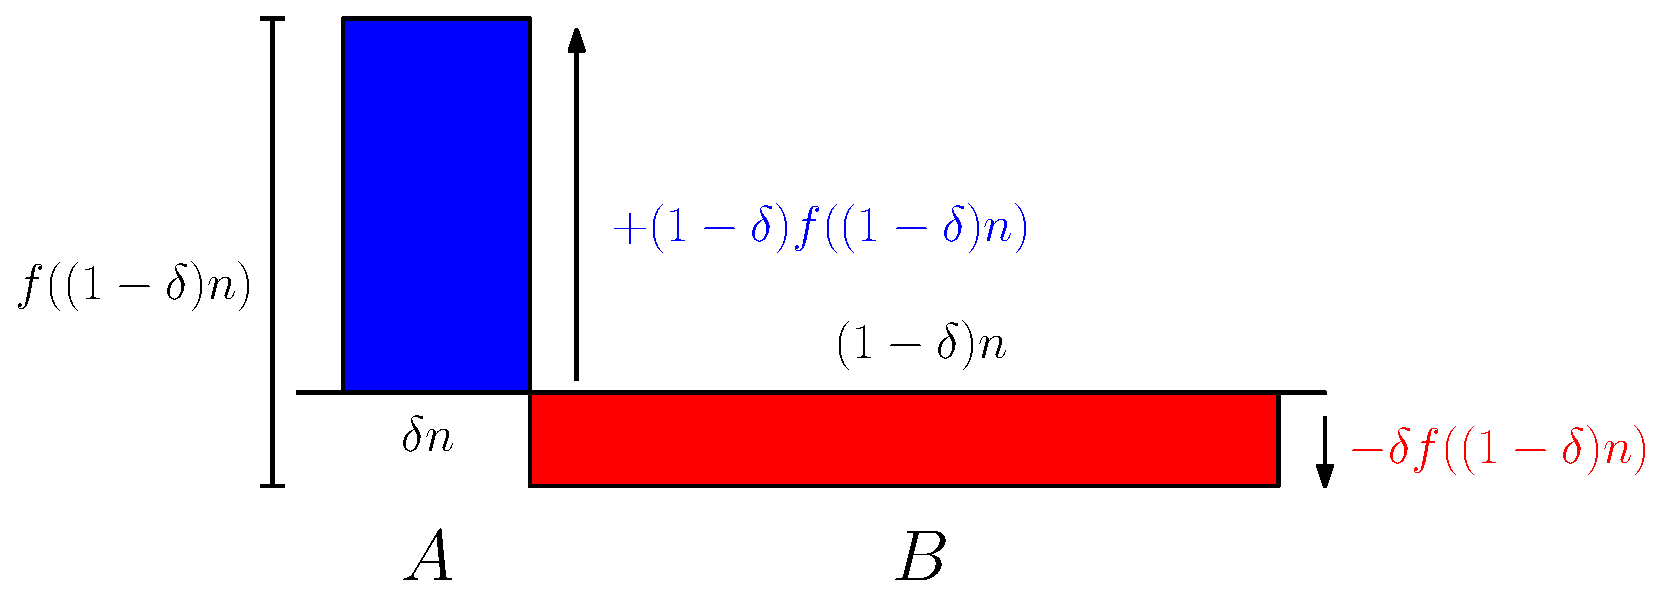
\includegraphics[width=\linewidth]{amplificationImgs/delta_one_minus_delta.eps}
\end{frame}

\begin{frame}[t]{Proof Sketch of Amplification Lemma}
  \begin{itemize}
    \item $A$ starts as the $\delta n$ fullest cups, $B$ as the $(1-\delta)n$ other cups.
    \item Repeatedly apply $f$ to $B$ and swap the cup with fill increased by $f(|B|)$ into $A$. 
    \item Decrease $p$ to $|A|$ and recurse on $A$.
  \end{itemize} 
\end{frame}

\begin{frame}[t]{Lower Bound against Adaptive Filler}
  By repeated amplification, using $\delta=\Theta(1)$, we get: 
  \begin{theorem}
    There is an adaptive filling strategy that achieves
    backlog $\Omega(n^{1-\epsilon})$ for constant
    $\epsilon > 0$ of our choice in running-time $2^{O(\log^2 n)}$.
  \end{theorem}
\end{frame}

\begin{frame}[t]{Lower Bound against Adaptive Filler}
  Setting $\delta = \Theta(1/n)$ -- which is quite extremal -- and recursively using
  the Amplification Lemma we prove:
  \begin{theorem}
    There is an adaptive filling strategy that achieves backlog $\Omega(n)$ in running-time $2^{O(n)}$.
  \end{theorem}
\end{frame}

\begin{frame}[t]{Lower Bound Intuitively}
  \vspace{0.5cm}
  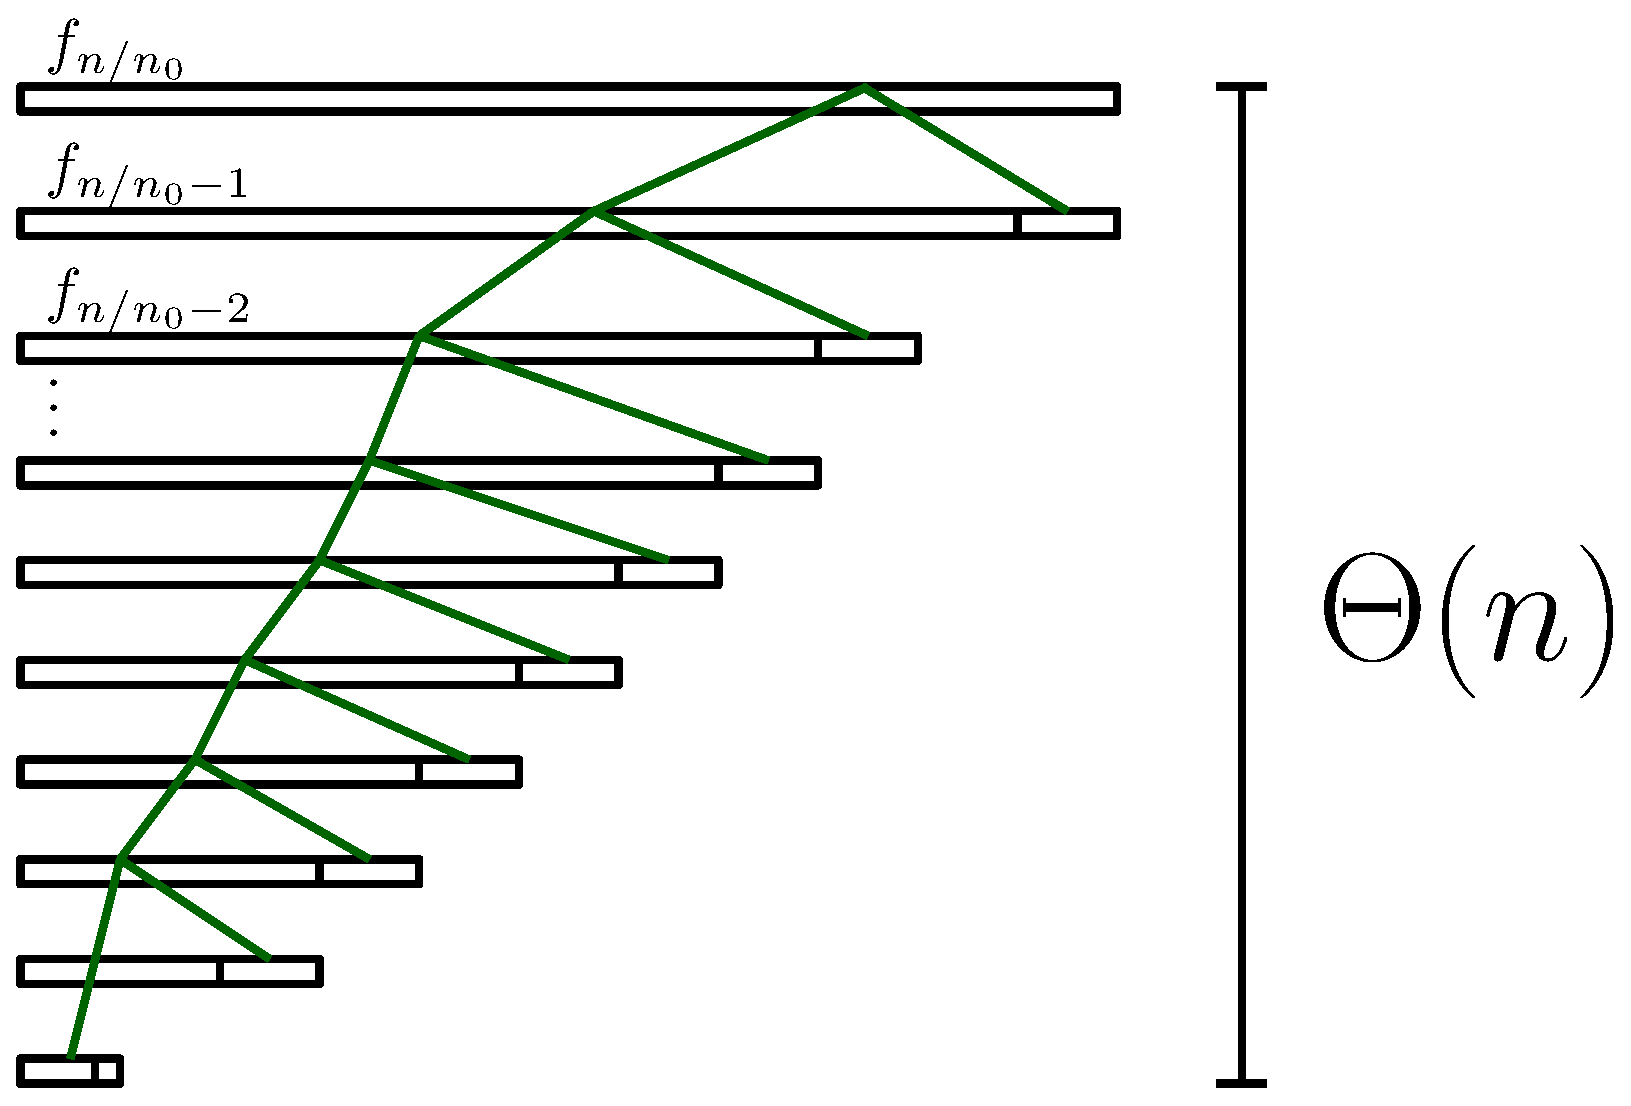
\includegraphics[width=0.7\linewidth]{amplificationImgs/expo_cor.eps}
\end{frame}

\begin{frame}[t]{Lower Bound Intuitively}
  \vspace{0.5cm}
  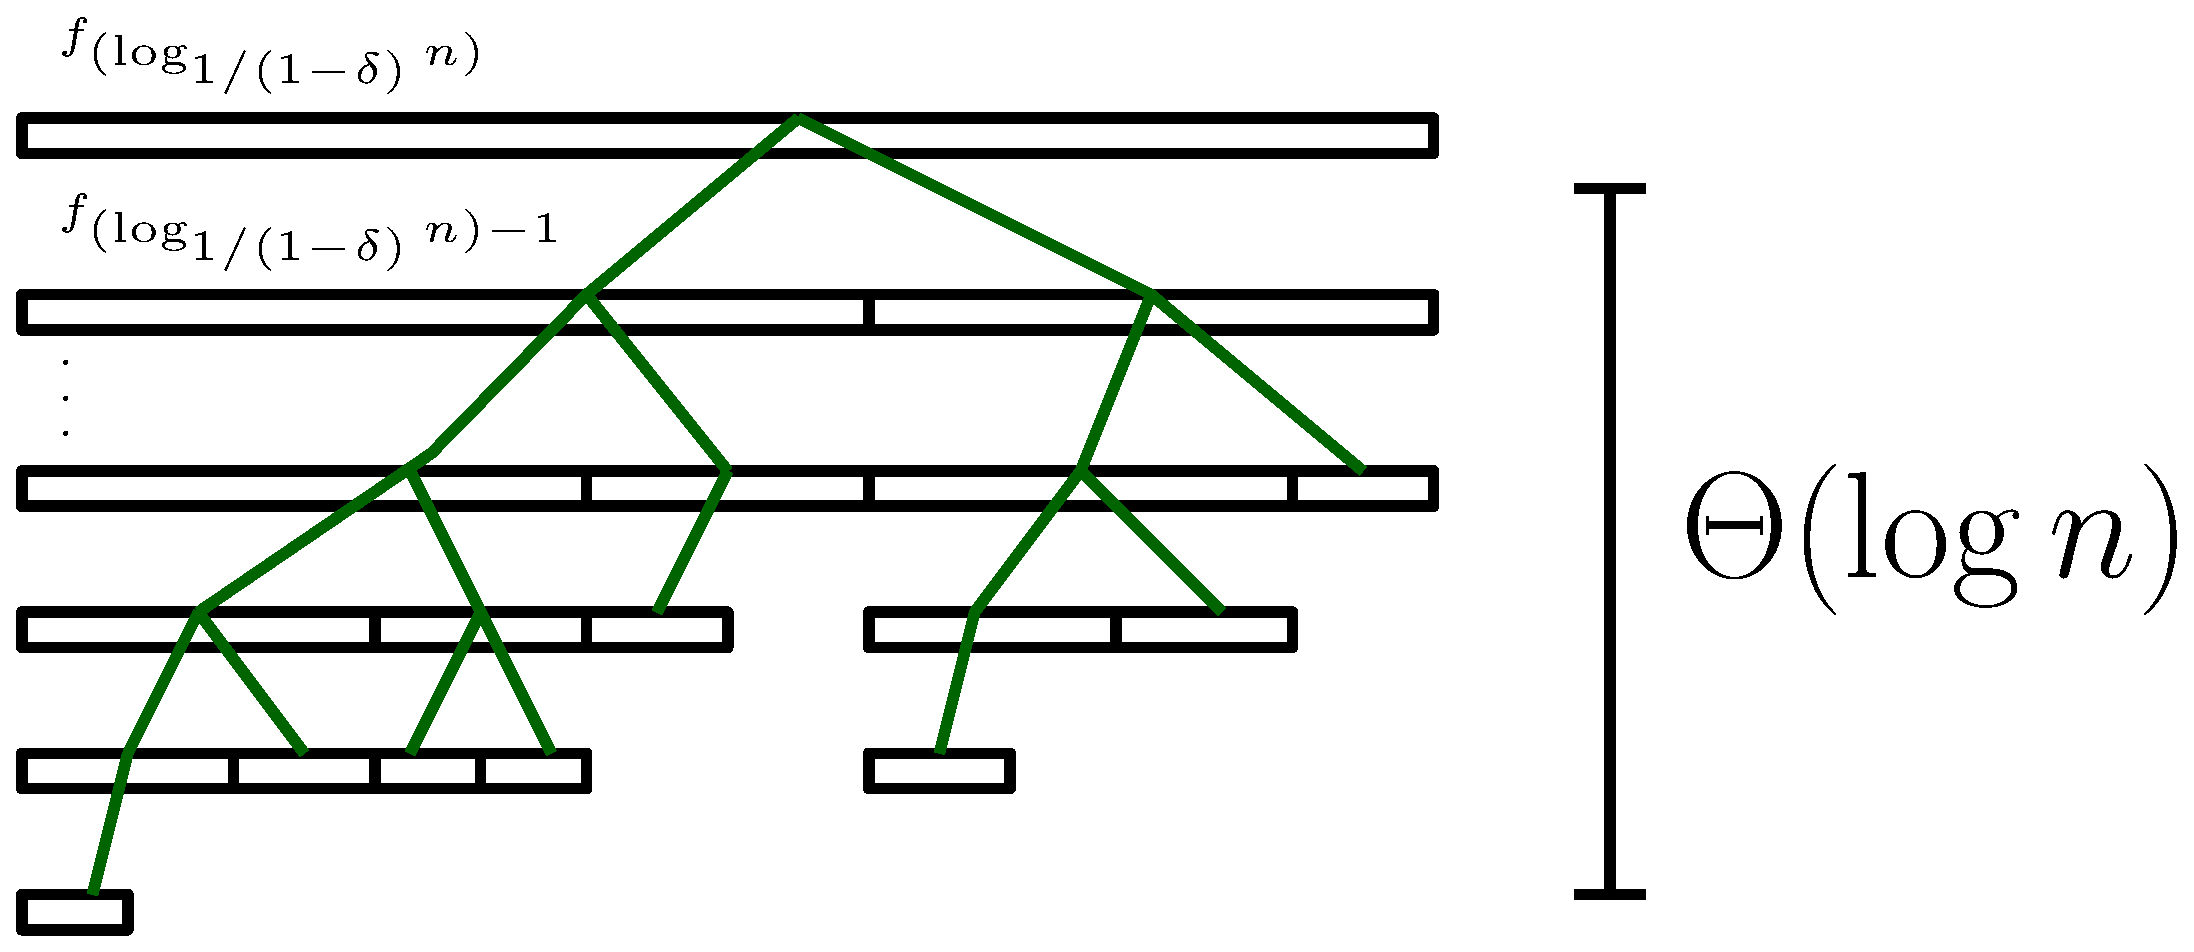
\includegraphics[width=0.7\linewidth]{amplificationImgs/quasipoly_cor.eps}
\end{frame}

\begin{frame}[t]{Upper Bound against Adaptive Filler}
  We prove a novel set of invariants:

  \begin{theorem}
    A greedy emptier maintains the invariant:
    $$\mu_k(S_t) \le 2n-k.$$
  \end{theorem}

  \vspace{0.3cm}
  In particular this implies that backlog is $$O(n).$$

  \vspace{0.3cm}
  Note: this matches our lower bound!
\end{frame}

\begin{frame}[t]{Upper Bound Proof Idea}
  Extremal fill configuration:
  \vspace{0.5cm}
  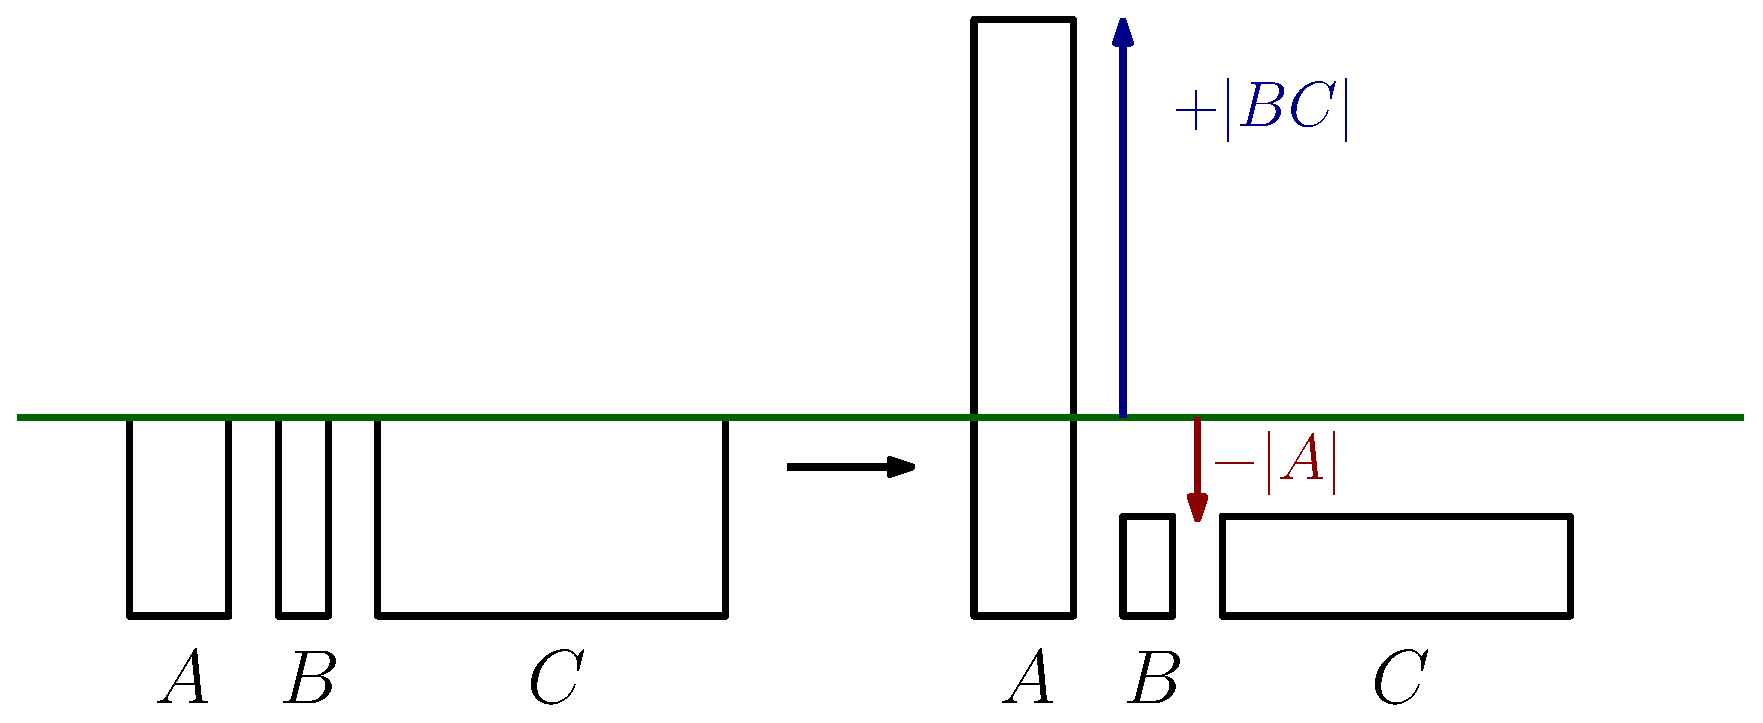
\includegraphics[width=\linewidth]{upperbound/upperboundpf.eps}
\end{frame}

\begin{frame}[t]{Lower Bound Against Oblivious Filler}
  Classically the emptier can do much better (e.g. $\log\log n$ vs $\log n$
  backlog) in the randomized setting.

  \vspace{0.5cm}

  In the variable-processor cup game--shockingly--an oblivious filler can
  achieve an identical lower bound for games of length $2^{\polylog(n)}$ 
  with probability at least $1-2^{-\polylog(n)}$, although only against \defn{greedy-like} emptiers.
\end{frame}

\begin{frame}[t]{Oblivious Filler: Constant Fill}
  Getting constant fill in a \emph{known} cup is hard now. Strategy:
  \begin{itemize}
    \item Play lots of single-processor cup games on constant numbers of cups
      blindly. Each succeeds with some constant probability.
    \item By a Chernoff Bound, with \emph{exponentially} good probability, i.e.
      $1-2^{-\Omega(n)}$, at least a constant fraction, say $nc$, of the single-processor
      cup games succeed.
    \item Set $p=nc$.
    \item Exploiting the greedy-like nature of the emptier fill a set of $nc$
      known cups while the emptier is forced to focus on the set of $nc$ with
      high fill.
    \item Recurse for a constant number of levels on the $nc$ cups with known high fill. 
  \end{itemize}
\end{frame}

\begin{frame}[t]{Oblivious Amplification Lemma}
Almost identical to the Adaptive Amplification Lemma!
  \begin{lemma}
    Given a strategy $f$, we can construct a new strategy that achieves backlog 
    $$f'(n) \ge \phi \cdot (1-\delta)\sum_{\ell=0}^L f((1-\delta)\delta^\ell n)$$
    for appropriate parameters $L\in\mathbb{N}, 0<\delta\ll 1/2$ and constant $\phi \in (0,1)$ of our choice.
  \end{lemma}
  Note that the Lemma is actually substantially more complicated than this: There are conditions
  on the starting configurations, everything succeeds with
  certain probabilities, the emptier must be greedy-like, we aren't discussing run-time here, and more.
\end{frame}

\begin{frame}[t]{Lower Bound Against Oblivious Filler}
  By a similar argument as for the adaptive case we have:
  \begin{theorem}
    There is an oblivious filling strategy that achieves backlog
    $\Omega(n^{1-\epsilon})$ for constant $\epsilon > 0$ with probability at
    least $1-2^{-\polylog(n)}$ in running time $2^{O(\log^2 n)}$.
  \end{theorem}
  Note that for the union bound to guarantee the appropriate probability the
  base case in our recursive argument has to be larger in the oblivious case
  than the adaptive case, but this doesn't harm our backlog result.
\end{frame}

\begin{frame}[t]{Open Questions}
  \begin{itemize}
    \item Can we extend the Oblivious lower-bound construction to work against arbitrary emptiers?
    \item Are there shorter more simple constructions?
  \end{itemize}
\end{frame}

\begin{frame}[t]{Acknowledgements}
  \begin{itemize}
    \item My mentor, William Kuszmaul!
    \item MIT PRIMES
    \item My Parents
 \end{itemize} 
\end{frame}

\end{document}
